\newcommand{\prob}{\rho}

\documentclass[tikz]{standalone}
\usetikzlibrary{arrows,shapes,automata,petri,positioning,calc}


\tikzset{
	state/.style={
		rectangle,
        rounded corners=5pt,
        draw,
		very thick,
		fill=orange!10,
		minimum height=5mm,
		minimum width=10mm,
	},
    link/.style={
        -angle 90,
        thick,
    }
}

\begin{document}
	
	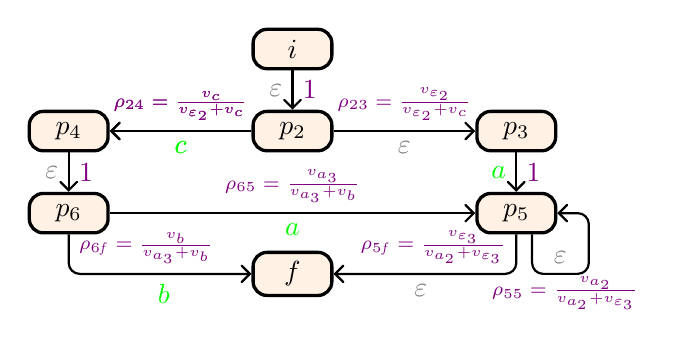
\begin{tikzpicture}[node distance=0.5cm and 1.8cm,>=stealth',bend angle=45,auto]
	
	
\node[state] (i) {$i$};
\node[state] (ii) [below=of i] {$p_2$};
\node[state] (iii) [right=of ii] {$p_3$};
\node[state] (iv) [left=of ii] {$p_4$};
\node[state] (v) [below=of iii] {$p_5$};
\node[state] (vi) [below=of iv] {$p_6$};
\node[below=of ii] (dot) {};
\node[state] (vii) [below=of dot] {$f$};

\draw[link] 
  (i) 
  -- 
  node[right]{\color{violet}$1$} 
  node[left]{\color{gray}$\varepsilon$}
  (ii);

\draw[link] 
  (ii) 
  -- 
  node[above,font=\scriptsize]{\color{violet}$\prob_{23} = \frac{v_{\varepsilon_2}}{v_{\varepsilon_2}+v_c}$} 
  node[below]{\color{gray}$\varepsilon$}
  (iii);

\draw[link] 
  (ii) 
  -- 
  node[above,font=\scriptsize]{\color{violet}$\prob_{24} = \frac{v_c}{v_{\varepsilon_2}+v_c}$} 
  node[below]{\color{green}$c$}
  (iv);

\draw[link] 
  (iii) 
  -- 
  node[right]{\color{violet}$1$} 
  node[left]{\color{green}$a$}
  (v);

\draw[link] 
  (iv) 
  -- 
  node[right]{\color{violet}$1$} 
  node[left]{\color{gray}$\varepsilon$}
  (vi);


\draw[link,rounded corners=4pt,] 
  (v) 
  |-
  node[above left,font=\scriptsize]{\color{violet}$\prob_{5\mathit{f}} = \frac{v_{\varepsilon_3}}{v_{a_2}+v_{\varepsilon_3}}$} 
  node[below left,xshift=-10mm]{\color{gray}$\varepsilon$}
  (vii);

\draw[link,rounded corners=4pt] 
  ($(v.south)+(2mm,0)$) 
  |-
  ($(v.south east)+(4mm,-5mm)$)  
  node[below,font=\scriptsize,yshift=1mm,xshift=-3mm]{\color{violet}$\prob_{55} = \frac{v_{a_2}}{v_{a_2}+v_{\varepsilon_3}}$} 
  node[above left,xshift=-1.5mm]{\color{gray}$\varepsilon$}
  |-
  (v.east);


\draw[link] 
  (ii) 
  -- 
  node[above,font=\scriptsize]{\color{violet}$\prob_{24} = \frac{v_c}{v_{\varepsilon_2}+v_c}$} 
  node[below]{\color{green}$c$}
  (iv);


\draw[link] 
  (vi) 
  -- 
  node[above,font=\scriptsize]{\color{violet}$\prob_{65} = \frac{v_{a_3}}{v_{a_3}+v_b}$} 
  node[below]{\color{green}$a$}
  (v);

\draw[link,rounded corners=4pt,] 
  (vi) 
  |-
  node[above right,font=\scriptsize]{\color{violet}$\prob_{6\mathit{f}} = \frac{v_{b}}{v_{a_3}+v_b}$} 
  node[below right,xshift=10mm]{\color{green}$b$}
  (vii);

\end{tikzpicture}
	
\end{document}